\documentclass{article}
\usepackage{tikz}
\usetikzlibrary{matrix} % LATEX and plain TEX when using TikZ
\begin{document}
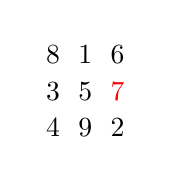
\begin{tikzpicture}[row 2 column 3/.style=red]
\matrix [matrix of nodes]
{
8 & 1 & 6 \\
3 & 5 & 7 \\
4 & 9 & 2 \\
};
\end{tikzpicture}

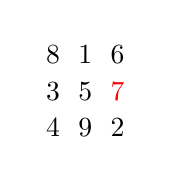
\begin{tikzpicture}
\matrix [matrix of nodes]
{
8 & 1 & 6 \\
3 & 5 & |[red]| 7 \\
4 & 9 & 2 \\
};
\end{tikzpicture}

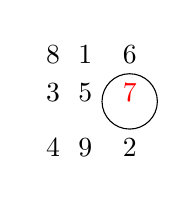
\begin{tikzpicture}
\matrix [matrix of nodes]
{
8 & 1 & 6 \\
3 & 5 & \node[red]{7}; \draw(0,0) circle(10pt);\\
4 & 9 & 2 \\
};
\end{tikzpicture}

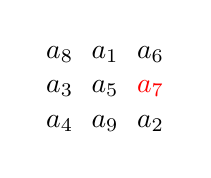
\begin{tikzpicture}
\matrix [matrix of math nodes]
{
a_8 & a_1 & a_6 \\
a_3 & a_5 & |[red]| a_7 \\
a_4 & a_9 & a_2 \\
};
\end{tikzpicture}

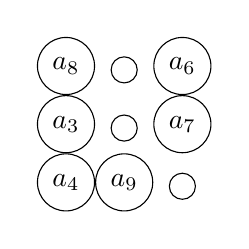
\begin{tikzpicture}
\matrix [matrix of math nodes,nodes={circle,draw},nodes in empty cells]
{
a_8 & & a_6 \\
a_3 & & a_7 \\
a_4 & a_9 & \\
};
\end{tikzpicture}

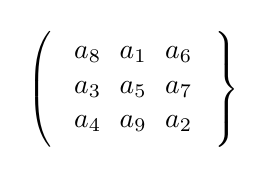
\begin{tikzpicture}
\matrix [matrix of math nodes,left delimiter=(,right delimiter=\}]
{
a_8 & a_1 & a_6 \\
a_3 & a_5 & a_7 \\
a_4 & a_9 & a_2 \\
};
\end{tikzpicture}

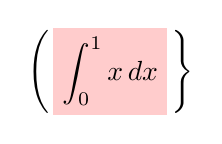
\begin{tikzpicture}
\node [fill=red!20,left delimiter=(,right delimiter=\}]
{$\displaystyle\int_0^1 x\,dx$};
\end{tikzpicture}

\end{document}
